\documentclass[a4paper]{report}

\usepackage{amsmath}
\usepackage{amsfonts}
\usepackage{graphicx}

\begin{document}

\section{Kinematics}
Kinematics is the science that studies the geometry of motion. It is restricted
to a purely geometrical description of motion by means of position, orientation
and their time derivatives.

Kinematic models are also fundamental to study the dynamics of the robots and
also to design controllers.

In robotics, kinematics helps to answer two questions:
\begin{itemize}
    \item{} Given a set of values for the different joint parameters (elbows,
        knees, etc.) where would the end effector (hand, foot, etc.) be located?
        This is know as forward kinematics.
    \item{} To position the effector in a particular place for instance to reach
        the door's knob or to place the foot in the right spot not fall, how
        should the joint parameters be adjusted? This is known as inverse kinematics.
\end{itemize}

The second problem is more interesting but it is also more complicated as multiple
solutions may exist for the same problem <reference>.


\section{Absolute and relative coordinate systems}
The study of kinematics begins by defining a global coordinate system, such
coordinate system will serve to describe the position of the robot and its
parts, as well as the position of all the other objects of interest in world.
This is known as the world coordinate system $\Sigma_W$, its origin can be
fixed anywhere in the world. When the position of an object is given in the
world coordinates it is common to refer to this position as the absolute
position, mathematically coordinates are represented by three dimensional vectors:
\begin{equation}
    \vec{p} = \begin{bmatrix}
        p_x\\
        p_y\\
        p_x\\
    \end{bmatrix}
\end{equation}

From time to time it is also convenient to have additional coordinate systems to
describe where things are located with respect to other objects in the world, for
example for a humanoid robot it may be useful to know where the door's knob is
located with respect to its hand or where the end of its arm is located with
respect to its elbow. In both examples the coordinate systems are attached to
a particular object (the hand, the elbow) and they move with that particular
object, these kind of coordinate systems are known as local coordinate systems.


\section{Homogeneous Transformations}
The use of multiple coordinate systems introduces a new problem, the same point
can be represented in multiple coordinate systems, a mechanism to transform the
coordinates of an object between coordinate systems is required. As shown by
<reference> such transformation can be performed with a homogeneous
transformation matrix, given a point $h$ with coordinates $^{b}\vec{p}_{h}$ in
a local coordinate system $\Sigma_b$ which has its $x_b$, $y_b$ and $z_b$ axis
rotated $\phi$, $\theta$ and $\psi$ degrees with respect to the $x_a$, $y_a$
and $z_a$ axis of another local coordinate system $\Sigma_{a}$, the coordinates
$^{a}\vec{p}_{h}$ of the point $h$ in $\Sigma_b$ is given by:

\begin{equation}
    \begin{bmatrix} ^{a}\vec{p}_{h} \\ 1 \end{bmatrix} = \,
        ^{a}\boldsymbol{T}_{b}
        \begin{bmatrix}
            ^{b}\vec{p}_{h} \\ 1
        \end{bmatrix} =
        \begin{bmatrix}
            ^{a}\boldsymbol{R}_{b} & ^{a}\vec{p}_{b} \\
            0 & 0 & 0 & 1
        \end{bmatrix}
        \begin{bmatrix}
            ^{b}\vec{p}_{h} \\
            1
        \end{bmatrix}
\end{equation}

Where:
\begin{itemize}
    \item{} $^{a}\boldsymbol{T}_{b}$ is a $4x4$ known as the homogeneous transformation matrix.
    \item{} $^{a}\boldsymbol{R}_{b}$ the rotation matrix, more on this below.
    \item{} $^{a}\vec{p}_{b}$ is the origin of $\Sigma_{b}$ viewed from $\Sigma_{a}$.
\end{itemize}

It's important to note that the homogeneous transformation matrix takes into
account both the rotational and the translational transformation.


\subsection{Rotation Matrix}
The rotation matrix can be seen in two different ways:
\begin{itemize}
    \item{} As a pure mathematical operator that rotates vectors <reference>
    \item{} As a matrix that represents the attitude of a local coordinate space
        and is defined as $\boldsymbol{R} = [e_x, e_y, e_z]$ as shown in figure
        \ref{fig:rotation_matrix}, where $e_x$, $e_y$ and $e_z$ are unit vectors.
\end{itemize}

\begin{figure}[htb!]
\begin{center}
    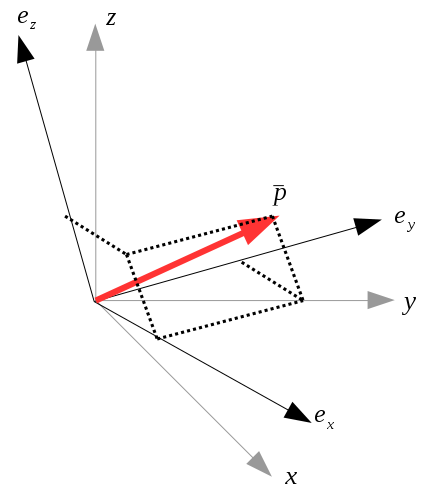
\includegraphics[width=0.5\textwidth]{./resources/rotation_matrix.png}
    \caption{Rotation matrix as the attitude of a coordinate system}
    \label{fig:rotation_matrix}
\end{center}
\end{figure}

The rotational matrix has another interesting property, from a linear algebra
point of view this matrix is orthogonal and it can be proved that <reference>:
\begin{equation}
    \boldsymbol{R}^{-1} = \boldsymbol{R}^{T}
\end{equation}

\subsection{Chain Rule}


\section{Angular Velocity}
By definition the velocity of a rigid body in the space is given by <reference>:
\begin{equation}
    \vec{v} = \vec{w} \times \vec{p}
\end{equation}

Where $\vec{w}$ is the angular velocity vector and $\vec{p}$ is a vector that
represents a given point $p$ on the surface of the rigid body. Just as position
vectors, velocity vectors can also be rotated:
\begin{equation}
\begin{split}
    \vec{v}\,' = \boldsymbol{R} \vec{v} \\
    \vec{p}\,' = \boldsymbol{R} \vec{p} \\
    \vec{w}\,' = \boldsymbol{R} \vec{w}
\end{split}
\end{equation}

thus:
\begin{equation}
\begin{split}
    \vec{v}\,' = \vec{w}\,' \times \vec{p}\,' \\
    \boldsymbol{R}\vec{v} = \boldsymbol{R} \vec{w} \times \boldsymbol{R} \vec{p}
\end{split}
\end{equation}



\end{document}
